Now that the relevant sentences for each entity have been extracted, we need to find out whether those sentences contain any information about our slots and find the value for those slots. In order to do this, we define the following properties of each slot:
\begin{itemize}
\item \textbf{TargetNERTypes:} set of possible NER Types that the slot value can have; NONE if it may not have an NER value
\item \textbf{Patterns:} we build patterns for each slot using the data provided to us and use those patterns to find slot values. 
\item \textbf{Threshold:} We associate a threshold with each slot which denotes above what confidence score we should predict a value for the slot.
\end{itemize}

Now, let’s talk about how we build the pattern sets and find confidence scores for each slot.
\subsection{Pattern finding for slots}
We use a combination of bootstrapping and rule based approaches to construct our patterns.
\begin{itemize}[label={}]
\item \textbf{Bootstrapping} \\
We use the bootstrapping method to find patterns for the different slots given to us as part of the problem. Since the index we created based on high recall filter had only those documents that mentioned the 170 entities, we created a separate index for around 21 days that indexed all the documents during this period (April 1 to 21, 2012). The choice of 21 days was made so that the dataset fit into the 1 TB hard disk size supported by the machines we used for indexing. The way the bootstrapping method works with is as follows:
\begin{enumerate}
\item We start with a manual seed-set, i.e. (entity, slot-value) pairs, for each slot
\item We extract documents that contain the entity and the slot-value and find the pattern connecting the entity and it’s slot value in the dependency parse of the sentence. 
\end{enumerate}

\begin{table*}[!ht]
\centering
\begin{tabular}{|c|c|}
\hline
Entity & Award \\
\hline
Meryl Streep & Oscar \\
Meryl Streep & Academy award \\
Meryl Streep & award \\
Geno Auriemma & Wooden Award \\
Anthony Davis & Naismith Award \\
Michel Hazanavicius & Oscar \\
Eli Sanders & Pulitzer prize \\ 
Mary Schmich & Pulitzer prize \\
Wesley Morris & Pulitzer prize \\
Hilary Mantel & Booker prize \\
Judea Pearl & Turing award \\
Saul Perlmutter & Nobel Prize \\
Tawakkol Karman & Nobel Prize \\ 
Leymah Gbowee & Nobel Prize \\
\hline
\end{tabular}
\caption{Seed set for the slot AwardsWon}
\label{tab:seedset_awardsWon}
\end{table*}

\begin{figure*}[t]
	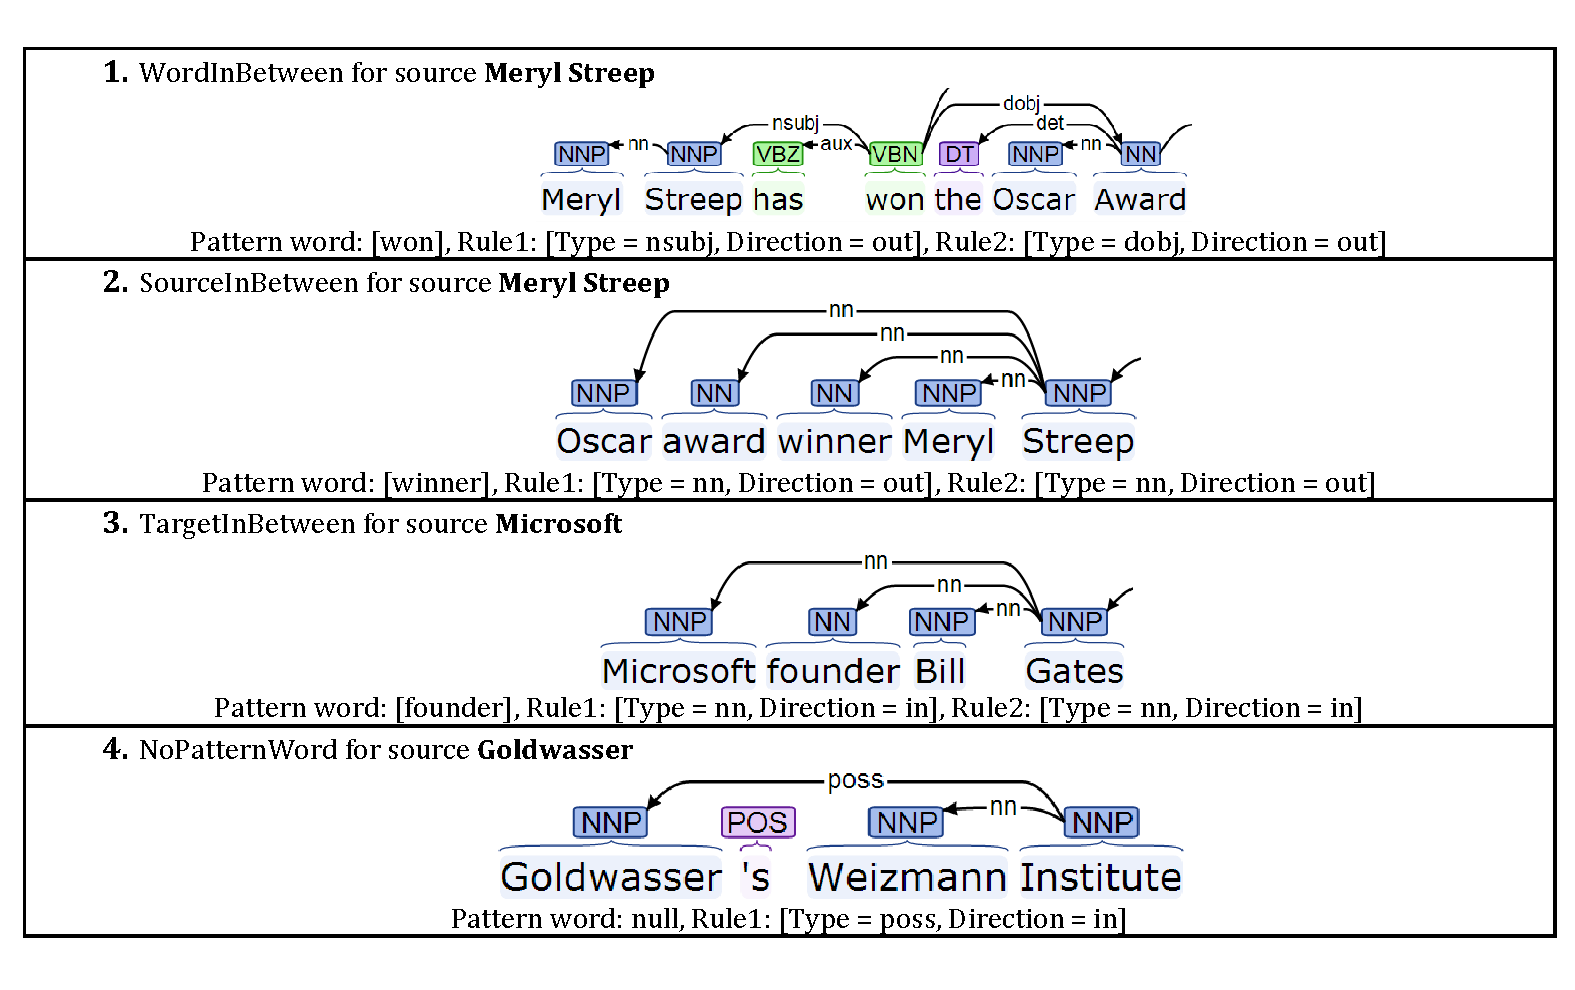
\includegraphics[width=0.97\textwidth]{Examples}
	\caption{Examples of different slot patterns found}
	\label{fig:slotpatternexamples}
\end{figure*}

The seed-set used for AwardsWon is shown in Table~\ref{tab:seedset_awardsWon}. The seed-set is constructed manually and can be (and most likely is) biased, despite our attempts to make it as representative as possible. We refer to the entity whose slot value has to be found as the source. The target is the desired slot-value we wish to extract from the sentence for any slot. And the pattern word is the word in the sentence that indicates the slot. For instance, the word ‘married’ is a pattern word for ‘AssociateOf’ relation between two people. Now, a pattern is defined by the pattern word and a set of at most two dependency rules that connect the source, target and the pattern word. The patterns we obtained using bootstrapping falls under four primary categories (based on the location of the pattern word in the path): 
\begin{enumerate}
\item \textbf{WordInBetween:} pattern word in the middle. These are the cases in which the pattern word appears in between the source and target entities in the dependency tree.Meryl Streep has won the Oscar Award for best actress at the Academy Award ceremony currently taking place at the Kodak Theatre in Hollywood.
\item \textbf{SourceInBetween:} In this case, the source word connects the target and the pattern word. Oscar award winner Mery Streep will talk in the ceremony on Monday.
\item \textbf{TargetInBetween:} In this case, the target word connects the source and the pattern word. Microsoft founder Bill Gates is popular for his acts of philanthropy.
\item \textbf{NoPatternWord:} source word connected directly to target by a dependency graph edge. Goldwasser's Weizmann Institute page.
\end{enumerate}
Some patterns found using bootstrapping for the slot EmployeeOf are shown in Table~\ref{tab:patterns_employeeOf}. 

\begin{table*}[ht]
\centering
\begin{tabular}{|c|c|c|c|}
\hline
Pattern Word & Pattern Type & Rule 1 & Rule 2 \\
\hline
ceo & WordInBetween & appos & appos \\
vp & SourceInBetween & nn & nn \\
engineer & WordInBetween & appos & prep\_at \\
reporter & SourceInBetween & nn & nn \\
spokesperson & WordInBetween & nsubj & prep\_at \\
\hline
\end{tabular}
\caption{Some patterns obtained using bootstrap for the slot EmployeeOf}
\label{tab:patterns_employeeOf}
\end{table*}

\textbf{Computing confidence thresholds} \\
The confidence with which we can tell that a pattern represents a desired slot depends on:
\begin{itemize}
\item How common it is used for a specific seed set entry? 
\item How prevalent it is across different seed sets? 
\end{itemize}

We don’t want to give a lot of importance to those patterns that just appear in one seed set. If we used absolute counts as weights, it could lead to one pattern that appeared for one seed set to get unusually high weight. So, we adopted the following strategy:
\begin{enumerate}
\item Normalize weights: The total weight for a seed set was fixed to 1 and each pattern found splits this weight proportionally.
\item Discard the lowest weight from across alll seed set. If a pattern appears just once across all the seed sets, it is likely that the pattern was not indicating the slot that we want to capture. So, we discount the lowest weight found.
\item Up weight frequent patterns: If a pattern appears in almost all seedsets, it should receive high confidence score. So, we upweight the total weight accumulated over the different patterns by multiplying it with the number of seed sets that extracted the patterns.
Overall formula for computing confidence
\end{enumerate}

\item \textbf{Rule based}\\
For some slots, the dependency parsing alone does not provide enough evidence. For example, for the slot Titles, the title can also be mentioned as a coreference to the entity in the sentence. For example, in the sentence, “Marissa Mayer, VP of Google, was also seen at the event.” Another such example is “Nobel Laureate Amartya Sen gave a lecture at the event”. Such values cannot be captured using the dependency parse of the sentence. Therefore, we use other rulesalso, in addition to the dependency parser, to find slot values.

It is important to note that the same strategy does not work for all kinds of documents. For example, while the sentences in the news articles are generally well formed, and therefore suitable for dependency parsing, the social documents can be very badly formed and therefore, not conducive to such strategies. The arxiv documents are another example where such dependency parses won’t work as the research papers have valuable associate information in the authors and references sections which cannot be obtained using a dependency parse. Therefore, we follow different strategies for different types of documents: for arxiv documents we exploit the systematic nature of paper writing and explicitly extract the information in different sections whereas for social documents, instead of relying on a dependency parse, we do a range query on our entity, the pattern word and a target word of appropriate entity type. News documents are generally well formed and we use the bootstrapped patterns directly on them.
\end{itemize}

\subsection{Finding slot values}
We use the patterns, rules and confidence thresholds computed in the previous step to find slot values in the set of relevant sentences. This is done using simple pattern matching, i.e. we find if a similar path exists in our sentence connecting our entity to a target word of the appropriate NER type. We do this for all sentences for the entity during the hour and accumulate the confidence scores of each pattern that matched and gave a slot value. In theory, this confidence score can be used to prune all slot values which lie below a certain threshold. However, in practice, we observed that the number of relevant sentences actually generating something useful for a slot was very low (\~1-2 per hour) and therefore, not significant enough for a threshold cutoff.

Another important step here is that of categorizing slot values into equivalence classes. As mentioned before, the same entity can be referred to in very different ways, these variations being even more prominent for facilities and organizations. However, when predicting slot values, we want to collapse all values which refer to the same entity into one equivalence class. Not only is this a requirement of the TREC-KBA submissions, it also helps in accumulating confidence scores for an equivalence class and making a better decision. We followed two major approaches to do this:
\begin{itemize}[label={}]
\item \textbf{Dictionary based}\\
We used the Google Cross Lingual Dictionary, which contains the different anchor texts used to point to a concept on wikipedia, to map a word to a wikipedia concept. While this system performed well, especially for facilities and organizations (it maps both Seagram Company and Seagram Inc Ltd. to Seagram, I.I.T. Delhi to Indian Institue of Technology Delhi, both Oscar and Oscar winner to Academy Award etc.), it is not the best way for us for two primary reasons. Firstly, because this method is dictionary based, it doesn’t take context into account. Therefore, even though William may refer to different people in different contexts, it will always map them to the same person. It is also not suitable for situations where the target entity may not have a corresponding wikipedia page. Secondly, for the purpose of our submission, we need only the equivalence class and not the concept representing the equivalence class.
\item \textbf{Approximate matching based} \\
Due to the drawbacks associated with the above method, we adopt a simple strategy where we simply find the k-gram jaccard similarity between two candidate values to predict whether they belong to the same equivalence class or not, the assumption again being that the document will have an explicit mention of the entity, and our system will therefore catch it.
\end{itemize}
